% vim: tw=80

\chapter{Conclusion}

In this thesis the measurement of triple-differential dijet cross sections has
been presented for the first time. The measurement has been performed using the
CMS detector at a center-of-mass energy of \SI{8}{\TeV} using the complete CMS
dataset collected in 2012 comprising \SI{19.71}{\fbinv}.

The cross sections were measured differentially in the average transverse
momentum of the dijet system, \ptavg, the boost of the dijet system, \yboost,
and half the rapidity separation of the dijets, \ystar. To correct the measured
cross sections for detector effects, they were unfolded using the iterative
d'Agostini algorithm. 

\begin{figure}[h!tbp]
    \centering
    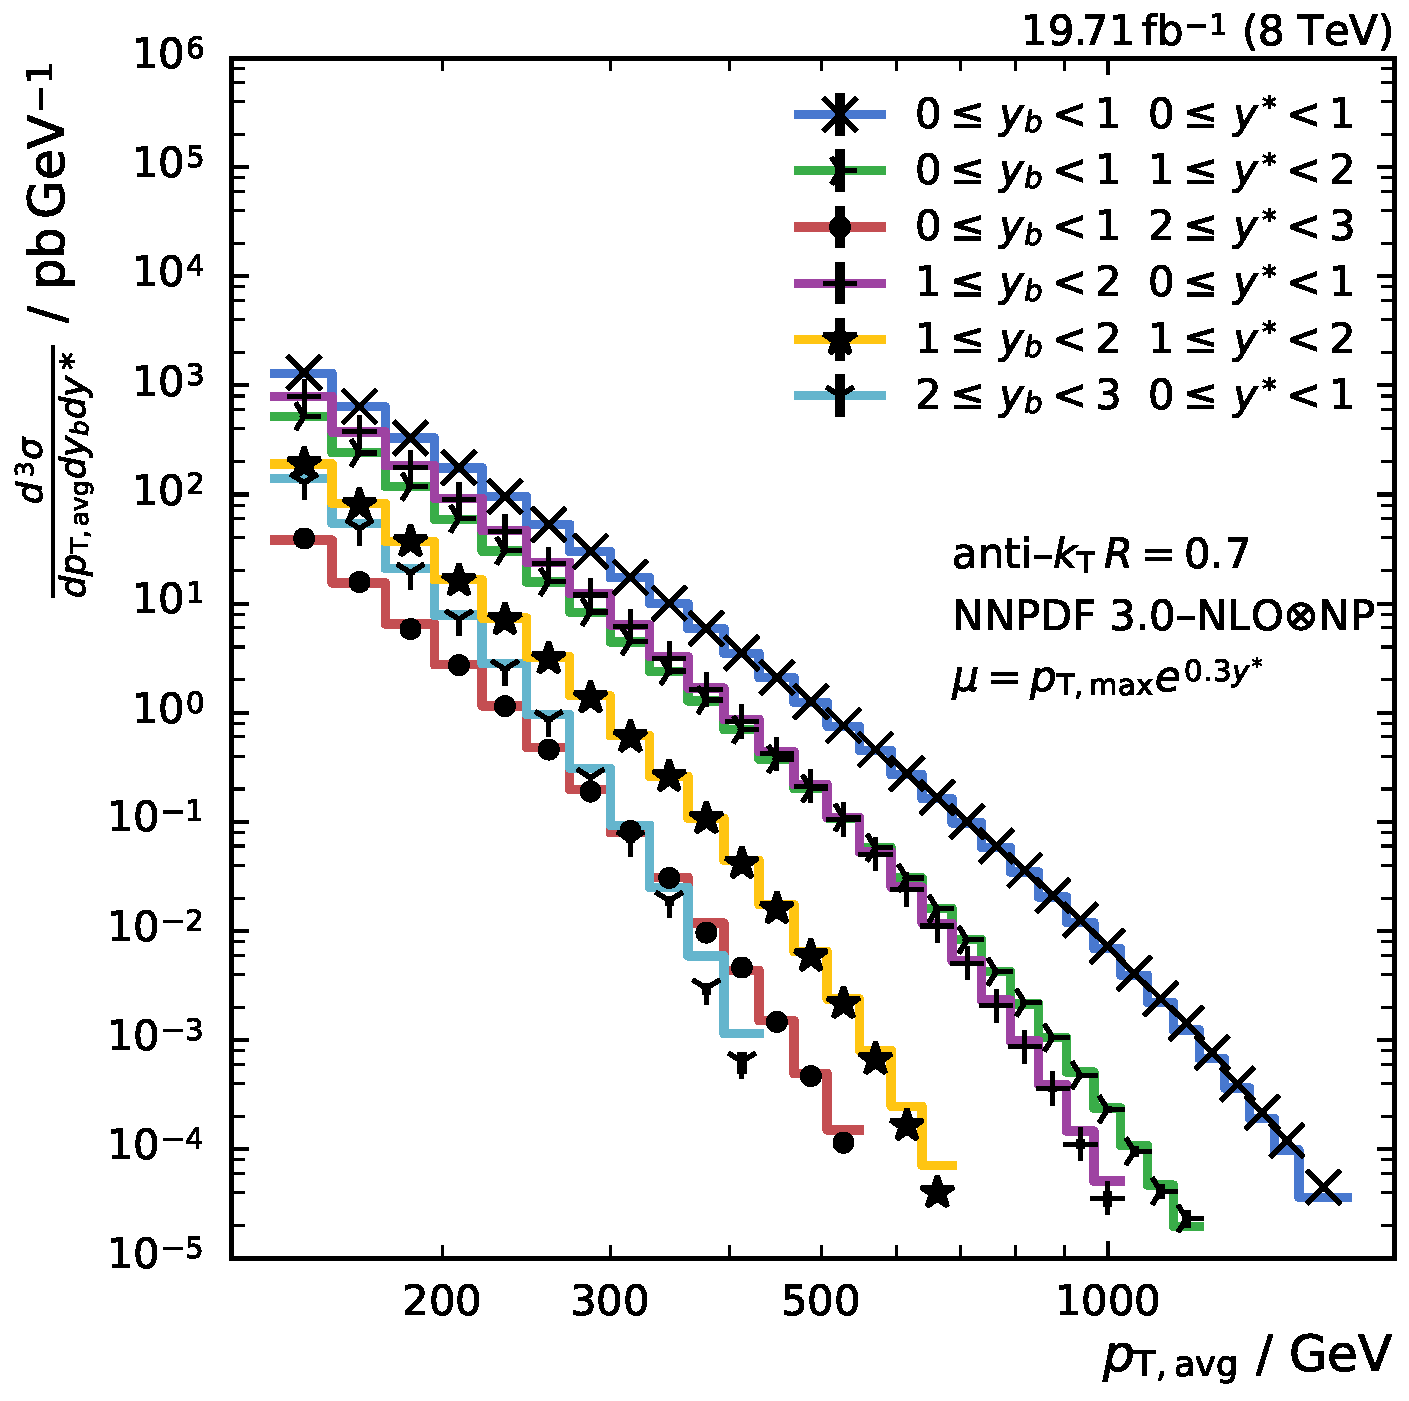
\includegraphics[width=0.45\textwidth]{figures/measurement/ptavg_spectrum.pdf}\hfill
    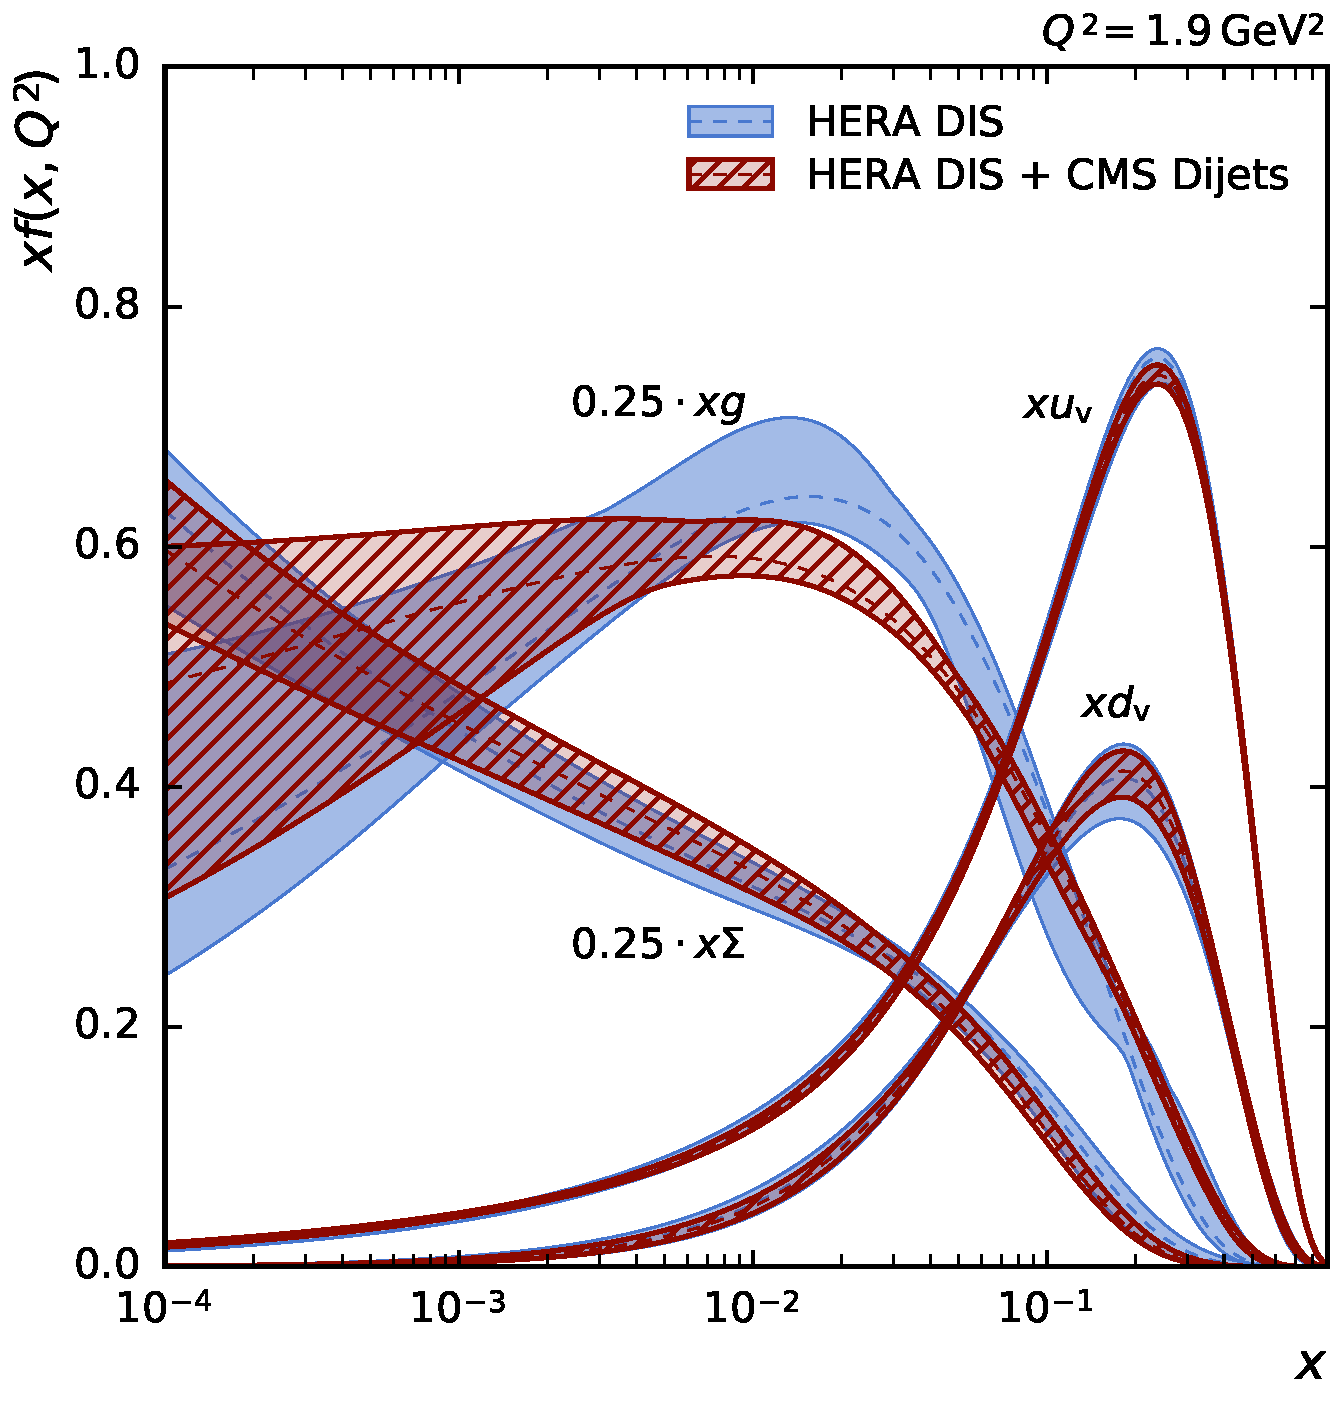
\includegraphics[width=0.45\textwidth]{figures/pdf_constraints/pdfcomp_direct_overview_1.9.pdf}
    \caption[Triple-differential dijet cross sections and PDF
    overview]{Left:
    The triple-differential dijet cross sections. The data points are indicated by black
    markers, the NLO theory prediction by colored lines. Right: Overview of
    fitted PDFs with and without including the triple-differential dijet
    measurement.}
    \label{fig:conclusion}
\end{figure}

Theoretical predictions have been calculated in pQCD at NLO accuracy and
corrected for non-perturbative effects. Fig.~\ref{fig:conclusion} left shows the
cross sections in the six studied \ystar and \yboost bins. It was found that the
data is well described by the predictions over many orders of magnitude. In
phase space regions containing boosted highly boosted dijet events, the data
discriminate between the predictions using different global PDF sets which at
the same time exhibit large uncertainties.

To demonstrate the sensitivity of the PDFs to the measured data, a combined PDF
fit of the HERA DIS and the dijet cross sections was performed. It was found
that the PDFs are improved when the dijet data are included and the
uncertainties of the PDFs, especially of the gluon PDF, is significantly
reduced. Fig.~\ref{fig:conclusion} right presents the PDF fits.

The strong coupling constant \asmz was determined by performing a simultaneous
fit of the PDFs and the strong coupling. The extracted value reads as

\begin{equation*}
  \asmz = 0.1188_{-0.0015}^{+0.0015}(\mathrm{exp})_{-0.0002}^{+0.0004}(\mathrm{mod})_{-0.0005}^{+0.0003}(\mathrm{par})_{-0.0010}^{+0.0029}(\mathrm{scale})
\end{equation*}

which is in good agreement with the world average value of the PDG. The
uncertainties on \asmz are dominated by the scale uncertainties which will
improve with the availability of NNLO calculations.
